\documentclass[a4paper,12pt]{article}\usepackage[]{graphicx}\usepackage[]{color}
%% maxwidth is the original width if it is less than linewidth
%% otherwise use linewidth (to make sure the graphics do not exceed the margin)
\makeatletter
\def\maxwidth{ %
  \ifdim\Gin@nat@width>\linewidth
    \linewidth
  \else
    \Gin@nat@width
  \fi
}
\makeatother

\definecolor{fgcolor}{rgb}{0.345, 0.345, 0.345}
\newcommand{\hlnum}[1]{\textcolor[rgb]{0.686,0.059,0.569}{#1}}%
\newcommand{\hlstr}[1]{\textcolor[rgb]{0.192,0.494,0.8}{#1}}%
\newcommand{\hlcom}[1]{\textcolor[rgb]{0.678,0.584,0.686}{\textit{#1}}}%
\newcommand{\hlopt}[1]{\textcolor[rgb]{0,0,0}{#1}}%
\newcommand{\hlstd}[1]{\textcolor[rgb]{0.345,0.345,0.345}{#1}}%
\newcommand{\hlkwa}[1]{\textcolor[rgb]{0.161,0.373,0.58}{\textbf{#1}}}%
\newcommand{\hlkwb}[1]{\textcolor[rgb]{0.69,0.353,0.396}{#1}}%
\newcommand{\hlkwc}[1]{\textcolor[rgb]{0.333,0.667,0.333}{#1}}%
\newcommand{\hlkwd}[1]{\textcolor[rgb]{0.737,0.353,0.396}{\textbf{#1}}}%

\usepackage{framed}
\makeatletter
\newenvironment{kframe}{%
 \def\at@end@of@kframe{}%
 \ifinner\ifhmode%
  \def\at@end@of@kframe{\end{minipage}}%
  \begin{minipage}{\columnwidth}%
 \fi\fi%
 \def\FrameCommand##1{\hskip\@totalleftmargin \hskip-\fboxsep
 \colorbox{shadecolor}{##1}\hskip-\fboxsep
     % There is no \\@totalrightmargin, so:
     \hskip-\linewidth \hskip-\@totalleftmargin \hskip\columnwidth}%
 \MakeFramed {\advance\hsize-\width
   \@totalleftmargin\z@ \linewidth\hsize
   \@setminipage}}%
 {\par\unskip\endMakeFramed%
 \at@end@of@kframe}
\makeatother

\definecolor{shadecolor}{rgb}{.97, .97, .97}
\definecolor{messagecolor}{rgb}{0, 0, 0}
\definecolor{warningcolor}{rgb}{1, 0, 1}
\definecolor{errorcolor}{rgb}{1, 0, 0}
\newenvironment{knitrout}{}{} % an empty environment to be redefined in TeX

\let\hlesc\hlstd \let\hlpps\hlstd \let\hllin\hlstd \let\hlslc\hlcom
\usepackage{alltt}

\usepackage[brazilian]{babel}
\usepackage[utf8]{inputenc}
\usepackage[T1]{fontenc}
\usepackage[margin=2.5cm]{geometry}
\usepackage{amsmath,amsfonts,amssymb,amsthm}
\usepackage{graphicx}
\usepackage{textcomp}
%\usepackage{url}
\usepackage{hyperref}
%\usepackage{fancyvrb}
%\usepackage{palatino,mathpazo}
%\usepackage[scaled]{helvet}
\usepackage[charter]{mathdesign} % serif: Bitstream Charter
\usepackage[scaled]{beramono} % truetype: Bistream Vera Sans Mono
\usepackage[scaled]{helvet}
\usepackage{float}

\usepackage{xspace}
\providecommand{\eg}{\textit{e.g}\xspace}
\providecommand{\R}{\textsf{R}\xspace}
\providecommand{\RStudio}{\textsf{RStudio}\xspace}

\title{Instalação do \textit{software} \R}
\author{Fernando de Pol Mayer \\
  LEA/IMEF/FURG \\
  \texttt{fernando.mayer@furg.br} \and Rodrigo Sant'Ana \\
  Instituto Albatroz \\
  \texttt{oc.rodrigosantana@gmail.com}}
\date{}

\hyphenation{e-la-bo-ra-das}
\IfFileExists{upquote.sty}{\usepackage{upquote}}{}
\begin{document}



\maketitle
\tableofcontents

\section{Introdução}

O \R é um programa para análise estatística de livre distribuição e de
código aberto. Isso significa que você pode baixar, instalar, repassar
para seus amigos e até mesmo alterar o código fonte de acordo com suas
necessidades. Ele pode ser instalado em diversas arquiteturas e sistemas
operacionais diferentes, incluindo Windows, Linux, Macintosh e
outros.

Este guia está dividido em duas seções, \textbf{Windows} e
\textbf{Linux}, e em cada uma existe uma versão ``rápida'' da instalação
(para os apressados), e uma versão ``longa'' (explicada em mais
detalhes).

\section{Windows}

\subsection{Instalação rápida}

\begin{enumerate}
\item \textbf{\R}:
  \url{http://cran-r.c3sl.ufpr.br/bin/windows/base/R-3.1.1-win.exe}
\item \textbf{\RStudio}:
  \url{http://download1.rstudio.org/RStudio-0.98.1079.exe}
\end{enumerate}

\textbf{Importante!} Instale nessa ordem: primeiro o \R e só depois o
\RStudio. O \RStudio é apenas uma interface para o \R, e por isso,
precisa encontrar a instalação do \R para poder ser instalado.

\subsection{Instalação longa}

\subsubsection{\R}

\begin{enumerate}
\item O primeiro passo é entrar na página do projeto \R em
\url{www.r-project.org}.
\item Do lado esquerdo da página clique sobre o link \texttt{CRAN}
  abaixo de \texttt{Download, Packages}.
\item Uma nova página com uma série de links irá se abrir. Esses links
  são chamados de ``espelhos'' e servem para que você possa escolher o
  local mais próximo de onde você está para fazer o download do
  programa. Vamos selecionar o espelho da Universidade Federal do
  Paraná. Procure o link \texttt{http://cran-r.c3sl.ufpr.br} e clique sobre
  ele.
\item Na seção \texttt{Download and Install R}, clique sobre o link
  \texttt{Download R for Windows} para baixar a versão para esse
  sistema.
\item Clique sobre o link \texttt{base}.
\item Clique sobre o link \texttt{Download R 3.1.1 for Windows} para
  fazer o download do arquivo \texttt{R-3.1.1-win.exe}.
\item A instalação segue o formato padrão de instalação de programas no
  Windows, e portanto não são necessários maiores detalhes.
\end{enumerate}

Após a instalação do \R, você pode abrir o programa clicando no ícone na
sua área de trabalho ou através do menu de programas. Se você já fez
isso, deve ter percebido que o programa tem uma aparência bem
``crua''. Esta interface, na verdade, é apenas a ``casca'' do \R, que
por ser uma linguagem de programação, não deve ter mesmo muitos recursos
gráficos. Seu grande potencial é através dos códigos que vamos
programar. Por esse motivo, os desenvolvedores do programa não gastam
tempo desenvolvendo uma inteface gráfica, mas sim na linguagem em si,
que é o mais importante.

Felizmente existem diversas pessoas que se empenharam em fazer
interfaces mais elaboradas para o \R, que não alteram como o programa
funciona (ou seja, não alteram em nada a linguagem), mas ajudam o
programador a ter um melhor controle e visualização sobre o código que
ele está escrevendo. Uma dessas interfaces é o
\href{http://www.sciviews.org/Tinn-R}{Tinn-R}, por exemplo. Há pouco
tempo atrás, uma nova interface chamada \RStudio foi lançada, com
diversas propriedades que ajudam muito quem está programando, e
principalmente, quem nunca usou o \R antes. Além disso, o \RStudio
funciona da mesma forma em todas as plataformas. Essa será a interface
que vamos utilizar.

\subsubsection{\RStudio}

\begin{enumerate}
\item Para baixar o \RStudio entre no endereço
  \url{www.rstudio.com}
\item Clique no link \texttt{Products > RStudio}
\item Clique em \texttt{RStudio Desktop}
\item Será exibida uma página com a recomendação para você baixar o
  \texttt{RStudio 0.98.1079 - Windows XP/Vista/7/8}
\item Clicando nesse link, você irá baixar o arquivo
  \texttt{RStudio-0.98.1079.exe}
\item Depois é só clicar e instalar da forma convencional do Windows
\end{enumerate}

Após a instalação, você pode abrir o \RStudio pelo ícone, e o \R estará
pronto para ser utilizado.

\section{Linux}

\subsection{Instalação rápida}
\label{sec:irl}

\begin{enumerate}
\item \textbf{\R}: Entre em \url{http://cran-r.c3sl.ufpr.br/bin/linux} e
  veja as instruções específicas para sua distribuição. As distribuições
  que já possuem pacotes pré-compilados para o \R estão listadas ali
  (Debian, RedHat [Fedora], Suse [OpenSuse], Ubuntu). Por exemplo, para
  instalar no Ubuntu, execute em um terminal
\begin{knitrout}\small
\definecolor{shadecolor}{rgb}{0.969, 0.969, 0.969}\color{fgcolor}\begin{kframe}
\noindent
\ttfamily
\hlstd{}\hlstd{\ \ }\hlstd{sudo\ apt}\hlopt{{-}}\hlstd{get\ }\hlkwc{install\ }\hlstd{r}\hlopt{{-}}\hlstd{base\ r}\hlopt{{-}}\hlstd{base}\hlopt{{-}}\hlstd{core}\hspace*{\fill}
\mbox{}
\normalfont
\normalsize
\end{kframe}
\end{knitrout}
  Se a sua distribuição não está listada ali, provavelmente será
  necessário compilar o código-fonte (veja na
  \hyperref[sec:ill]{Instalação longa} abaixo).
\item \textbf{\RStudio}: Entre em
  \url{http://www.rstudio.com/products/rstudio/download}
  e procure um pacote
  pré-compilado para sua distribuição. Normalmente, após baixar esse
  pacote, a instalação pode ser executada apenas abrindo o arquivo. Em
  todo caso, tomando o Ubuntu novamente como exemplo, a instalação pode
  ser feita também via terminal com
\begin{knitrout}\small
\definecolor{shadecolor}{rgb}{0.969, 0.969, 0.969}\color{fgcolor}\begin{kframe}
\noindent
\ttfamily
\hlstd{}\hlstd{\ \ }\hlstd{sudo\ dpkg\ }\hlopt{{-}}\hlstd{i\ rstudio}\hlopt{{-}}\hlstd{}\hlnum{0.98.1079}\hlstd{}\hlopt{{-}}\hlstd{amd64.deb}\hspace*{\fill}
\mbox{}
\normalfont
\normalsize
\end{kframe}
\end{knitrout}
  Note que o arquivo \texttt{rstudio-0.98.1079-amd64.deb} é uma versão
  específica para o Ubuntu 64 bits, e você deve estar no diretório onde
  o arquivo foi baixado (use o comando \texttt{cd} para mudar
  diretórios).

\end{enumerate}

\textbf{Importante!} Instale nessa ordem: primeiro o \R e só depois o
\RStudio. O \RStudio é apenas uma interface para o \R, e por isso,
precisa encontrar a instalação do \R para poder ser instalado.

\subsection{Instalação longa}
\label{sec:ill}

\subsubsection{\R}

Se você não encontrou um pacote pré-compilado do \R para sua
distribuição específica, ou, se você quer instalar o \R compilando o
código-fonte, siga as instruções abaixo. Compilar o código-fonte oferece
uma série de vantagens como a personalização da instalação, e um ganho
de performance do programa quando comparado com versões pré-compiladas.

\begin{enumerate}
\item O primeiro passo é entrar na página do projeto \R em
\url{www.r-project.org}.
\item Do lado esquerdo da página clique sobre o link \texttt{CRAN}
  abaixo de \texttt{Download, Packages}.
\item Uma nova página com uma série de links irá se abrir. Esses links
  são chamados de ``espelhos'' e servem para que você possa escolher o
  local mais próximo de onde você está para fazer o download do
  programa. Vamos selecionar o espelho da Universidade Federal do
  Paraná. Procure o link \texttt{http://cran-r.c3sl.ufpr.br} e clique sobre
  ele.
\item Na seção \texttt{Source Code for all Platforms}, baixe o arquivo
  \texttt{R-2.15.2.tar.gz} (link direto:
  \url{http://cran-r.c3sl.ufpr.br/src/base/R-3/R-3.1.1.tar.gz})
\item Coloque esse arquivo em um diretório de sua escolha, abra um
  terminal e acesse esse diretório (usando \texttt{cd}). Por exemplo, se
  o arquivo estiver dentro de um diretório chamado \texttt{Programas},
  no diretório padrão do usuário
\begin{knitrout}\small
\definecolor{shadecolor}{rgb}{0.969, 0.969, 0.969}\color{fgcolor}\begin{kframe}
\noindent
\ttfamily
\hlstd{}\hlstd{\ \ }\hlstd{}\hlkwb{cd\ }\hlstd{Programas}\hlopt{/}\hlstd{}\hspace*{\fill}
\mbox{}
\normalfont
\normalsize
\end{kframe}
\end{knitrout}
\item Descompacte o arquivo com o comando \texttt{tar}
\begin{knitrout}\small
\definecolor{shadecolor}{rgb}{0.969, 0.969, 0.969}\color{fgcolor}\begin{kframe}
\noindent
\ttfamily
\hlstd{}\hlstd{\ \ }\hlstd{}\hlkwc{tar\ }\hlstd{}\hlopt{{-}}\hlstd{zxvf\ R}\hlopt{{-}}\hlstd{}\hlnum{3.1.1}\hlstd{.}\hlkwc{tar}\hlstd{.gz}\hspace*{\fill}
\mbox{}
\normalfont
\normalsize
\end{kframe}
\end{knitrout}
  Isso irá criar um diretório chamado \texttt{R-3.1.1}. Entre nesse
  diretório
\begin{knitrout}\small
\definecolor{shadecolor}{rgb}{0.969, 0.969, 0.969}\color{fgcolor}\begin{kframe}
\noindent
\ttfamily
\hlstd{}\hlstd{\ \ }\hlstd{}\hlkwb{cd\ }\hlstd{R}\hlopt{{-}}\hlstd{}\hlnum{3.1.1}\hlstd{}\hspace*{\fill}
\mbox{}
\normalfont
\normalsize
\end{kframe}
\end{knitrout}
\item Agora você pode configurar (\texttt{configure}), compilar
  (\texttt{make}), verificar a compilação (\texttt{make check-all})
  (esse processo pode ser demorado), e finalmente instalar (\texttt{make
  install}). O processo todo fica assim
\begin{knitrout}\small
\definecolor{shadecolor}{rgb}{0.969, 0.969, 0.969}\color{fgcolor}\begin{kframe}
\noindent
\ttfamily
\hlstd{}\hlstd{\ \ }\hlstd{.}\hlopt{/}\hlstd{configure\hspace*{\fill}\\
}\hlstd{\ \ }\hlstd{}\hlkwc{make}\hspace*{\fill}\\
\hlstd{}\hlstd{\ \ }\hlstd{}\hlkwc{make\ }\hlstd{check}\hlopt{{-}}\hlstd{all\hspace*{\fill}\\
}\hlstd{\ \ }\hlstd{sudo\ }\hlkwc{make\ install}\hlstd{}\hspace*{\fill}
\mbox{}
\normalfont
\normalsize
\end{kframe}
\end{knitrout}
  Detalhe: se você for realmente utilizar o \RStudio como interface no
  Linux, é necessário compilar o \R como um \textit{shared
    library}. Para isso, substitua a primeira linha acima por
\begin{knitrout}\small
\definecolor{shadecolor}{rgb}{0.969, 0.969, 0.969}\color{fgcolor}\begin{kframe}
\noindent
\ttfamily
\hlstd{}\hlstd{\ \ }\hlstd{.}\hlopt{/}\hlstd{configure\ }\hlopt{{-}{-}}\hlstd{}\hlkwb{enable}\hlstd{}\hlopt{{-}}\hlstd{R}\hlopt{{-}}\hlstd{shlib}\hspace*{\fill}
\mbox{}
\normalfont
\normalsize
\end{kframe}
\end{knitrout}
  e continue com os demais comandos.
\item No Linux, o \R não tem interface alguma, ele é um programa que
  roda no terminal. Por isso, você pode verificar a instalação apenas digitando
\begin{knitrout}\small
\definecolor{shadecolor}{rgb}{0.969, 0.969, 0.969}\color{fgcolor}\begin{kframe}
\noindent
\ttfamily
\hlstd{}\hlstd{\ \ }\hlstd{R}\hspace*{\fill}
\mbox{}
\normalfont
\normalsize
\end{kframe}
\end{knitrout}
  no terminal.
\end{enumerate}

Como por padrão o \R não tem uma interface no Linux, você pode optar por
muitas alternativas como o \href{http://ess.r-project.org}{ESS} (Emacs
Speaks Statistics) para o
\href{http://www.gnu.org/software/emacs/}{Emacs}, o
\href{http://www.lepem.ufc.br/jaa/r-plugin.html}{Vim-R-plugin} para o
\href{http://www.vim.org}{Vim}, ou o
\href{http://rgedit.sourceforge.net}{RGedit} para o
\href{http://projects.gnome.org/gedit}{Gedit}.

Além destas opções mais tradicionais, o \RStudio também têm suporta para
Linux, e funciona exatamente da mesma forma como no Windows.

\subsubsection{\RStudio}

\begin{enumerate}
\item Para baixar o \RStudio entre no endereço
  \url{www.rstudio.org}
\item Clique no link \texttt{Products > RStudio}
\item Clique em \texttt{RStudio Desktop}
\item Será exibida uma página com a recomendação para você baixar o
  \RStudio de acordo com a distribuição que você estiver usando
\item Clique no link recomendado para baixar o arquivo
\item Normalmente clicando duas vezes sobre o arquivo, o programa já
  será instalado. Um exemplo de instlação via terminal no Ubuntu está na
  \hyperref[sec:irl]{Instalação rápida} acima.
\end{enumerate}

Após a instalação, você pode abrir o \RStudio pelo ícone, e o \R estará
pronto para ser utilizado.

\section{Usando \R e \RStudio}

Após abrir o \RStudio você vai se deparar com uma interface como essa:

\begin{figure}[H]
  \centering
  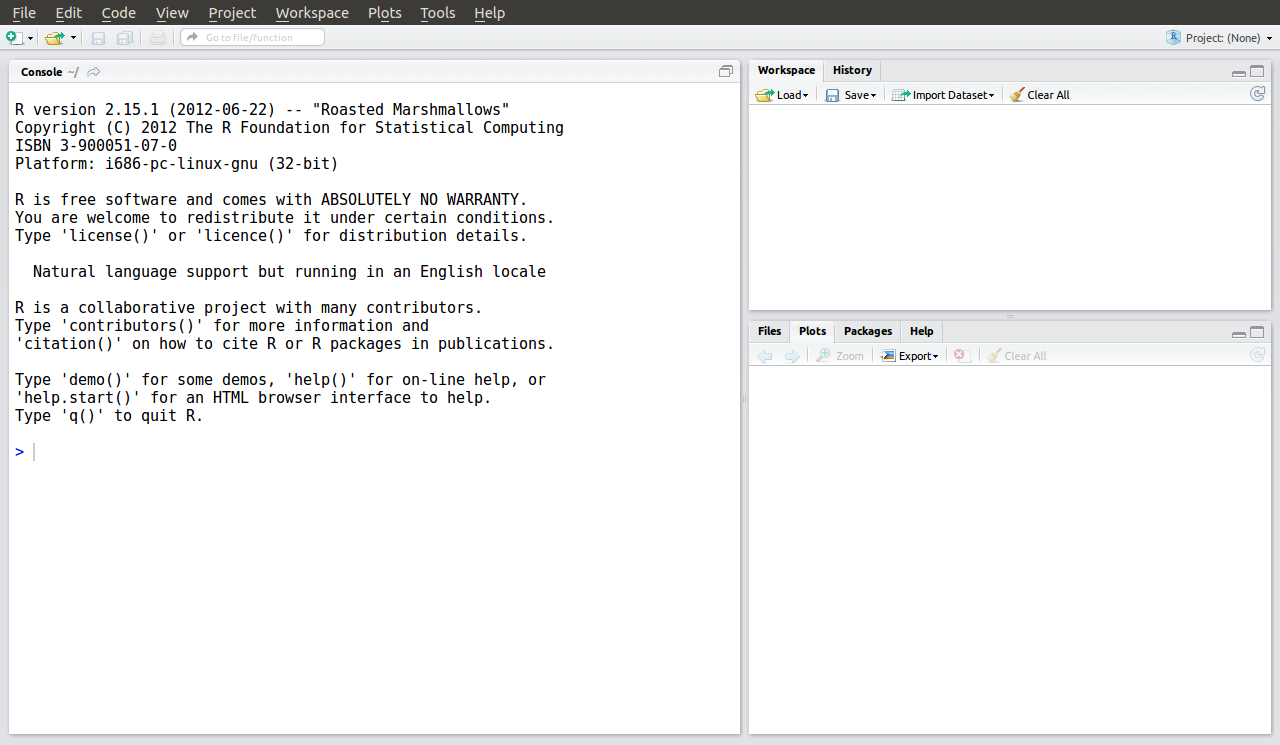
\includegraphics[width=\textwidth]{figure/RStudio_002}
\end{figure}

\clearpage

A parte esquerda do programa é chamada de \textsf{Console}, onde os
comandos do \R serão executados. Sempre que \RStudio for iniciado, uma
mensagem como essa deverá aparecer:

%<<eval=FALSE>>=
%R version 2.15.1 (2012-06-22) -- "Roasted Marshmallows"
%Copyright (C) 2012 The R Foundation for Statistical Computing
%ISBN 3-900051-07-0
%Platform: x86_64-unknown-linux-gnu (64-bit)
%
%R is free software and comes with ABSOLUTELY NO WARRANTY.
%You are welcome to redistribute it under certain conditions.
%Type 'license()' or 'licence()' for distribution details.
%
%  Natural language support but running in an English locale
%
%R is a collaborative project with many contributors.
%Type 'contributors()' for more information and
%'citation()' on how to cite R or R packages in publications.
%
%Type 'demo()' for some demos, 'help()' for on-line help, or
%'help.start()' for an HTML browser interface to help.
%Type 'q()' to quit R.
%
%>
%@

\begin{figure}[H]
  \centering
  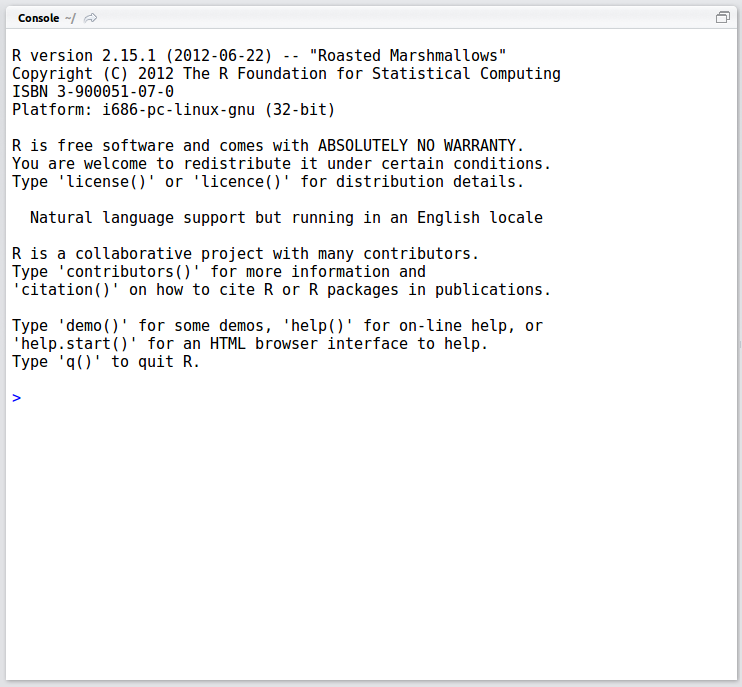
\includegraphics[width=.7\textwidth]{figure/Selection_011}
\end{figure}

Talvez o seu esteja em português, mas a mensagem é a mesma. Se apareceu
isso, o \R está funcionando corretamente dentro do
\RStudio. Lembre-se que o \RStudio é apenas uma interface
gráfica, e o \R está rodendo ``dentro'' dela.  O símbolo \texttt{>}
sinaliza que o \R está esperando para executar algum comando.

Antes de começar a fazer qualquer coisa no \R, é recomendado
``direcioná-lo'' para um diretório de trabalho (\textit{working
  directory}). É neste diretório que todos os arquivos que você criar
(\eg gráficos, scripts), ou aqueles que quiser importar para o \R (\eg
bases de dados) ficarão armazenados. Para fazer esse direcionamento no
\RStudio, clique no menu em \textsf{Tools $\rightarrow$ Set Working
  Directory $\rightarrow$ Choose Directory}, como na figura abaixo:

\begin{figure}[H]
  \centering
  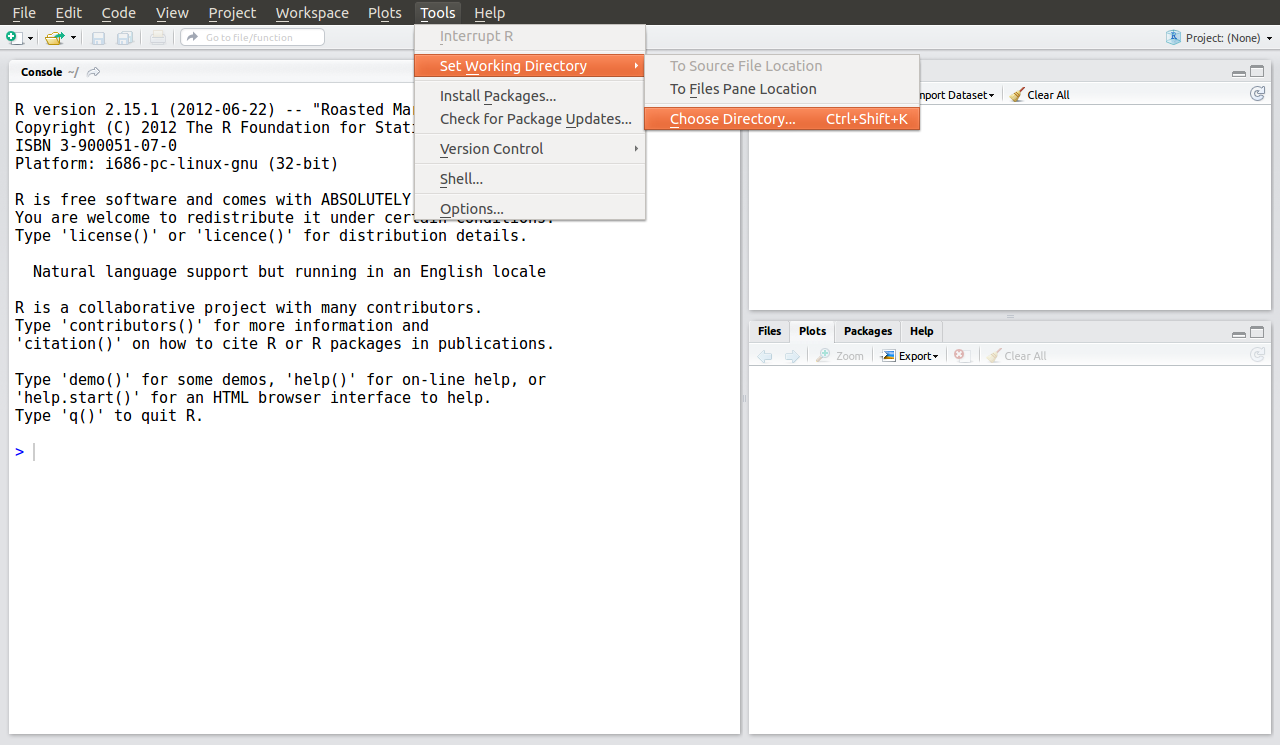
\includegraphics[width=\textwidth]{figure/RStudio_005}
\end{figure}
Na janela que irá abrir, selecione um diretório (ou crie um), clique em
\textsf{Abrir}, e automaticamente o \R vai executar no \textsf{Console}
o comando \texttt{setwd()} (que significa ``\texttt{set} \texttt{w}orking
\texttt{d}irectory''). Dentro do parênteses da função, e entre aspas,
deverá aparecer o caminho para o diretório que você especificou. No
exemplo abaixo, o diretório selecionado foi \texttt{/home/fernando/R}
(ou \verb|~/R| no Linux).

\begin{figure}[H]
  \centering
  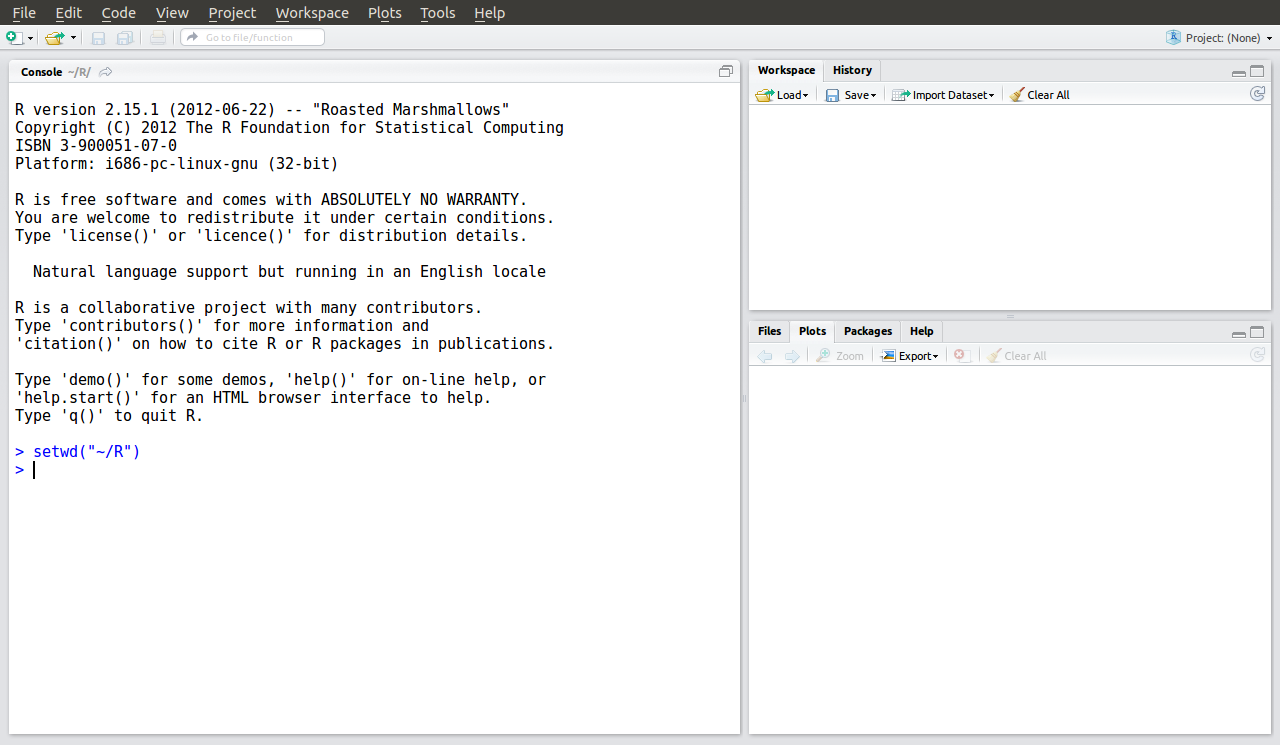
\includegraphics[width=\textwidth]{figure/RStudio_006}
\end{figure}

O próximo passo é utilizar o editor de scripts para entrar
comandos. Obviamente você pode digitar comandos diretamente no
\textsf{Console}, que o \R irá executá-los, mas à medida que os comandos
vão aumentando, fica mais fácil se você salvá-los em um arquivo. Para
isso clique no menu em \textsf{File $\rightarrow$ New $\rightarrow$ R
  Script}, como na figura abaixo:

\begin{figure}[H]
  \centering
  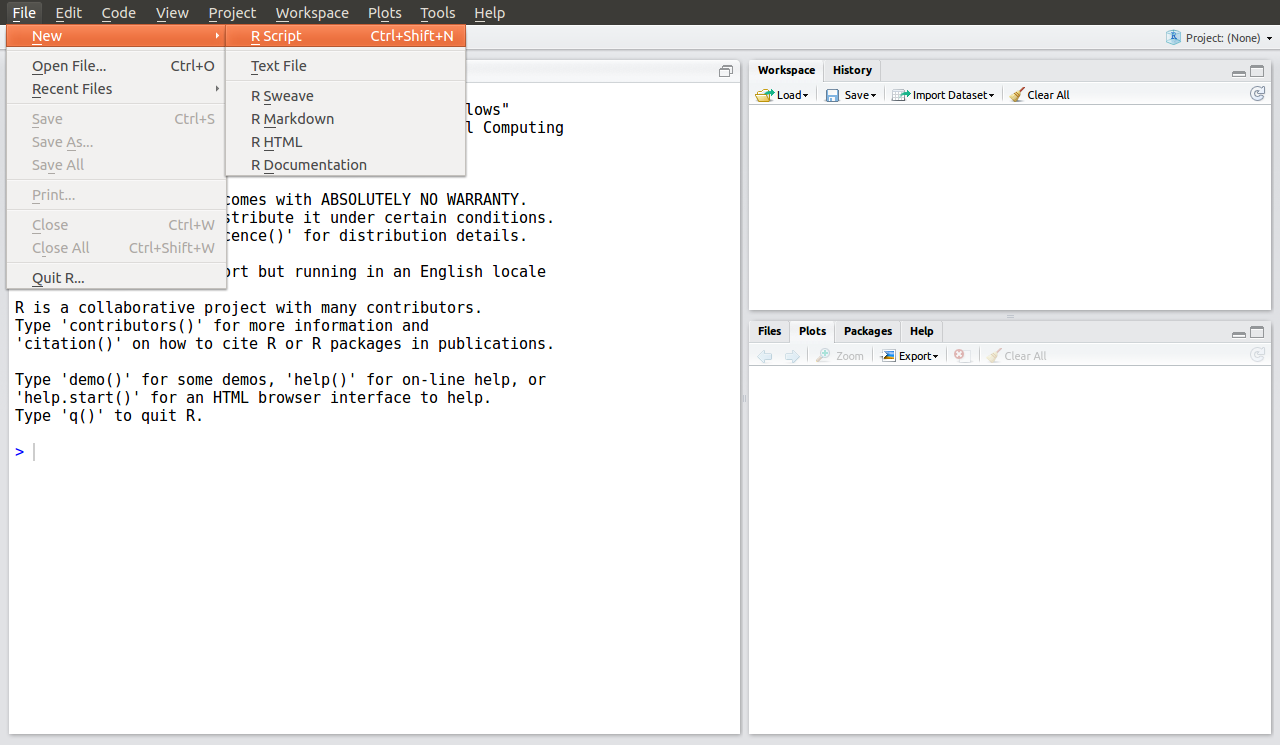
\includegraphics[width=\textwidth]{figure/RStudio_010}
\end{figure}

Esse processo irá abrir uma nova ``janela'' dentro do \RStudio, acima do
\textsf{Console}, como na figura:

\begin{figure}[H]
  \centering
  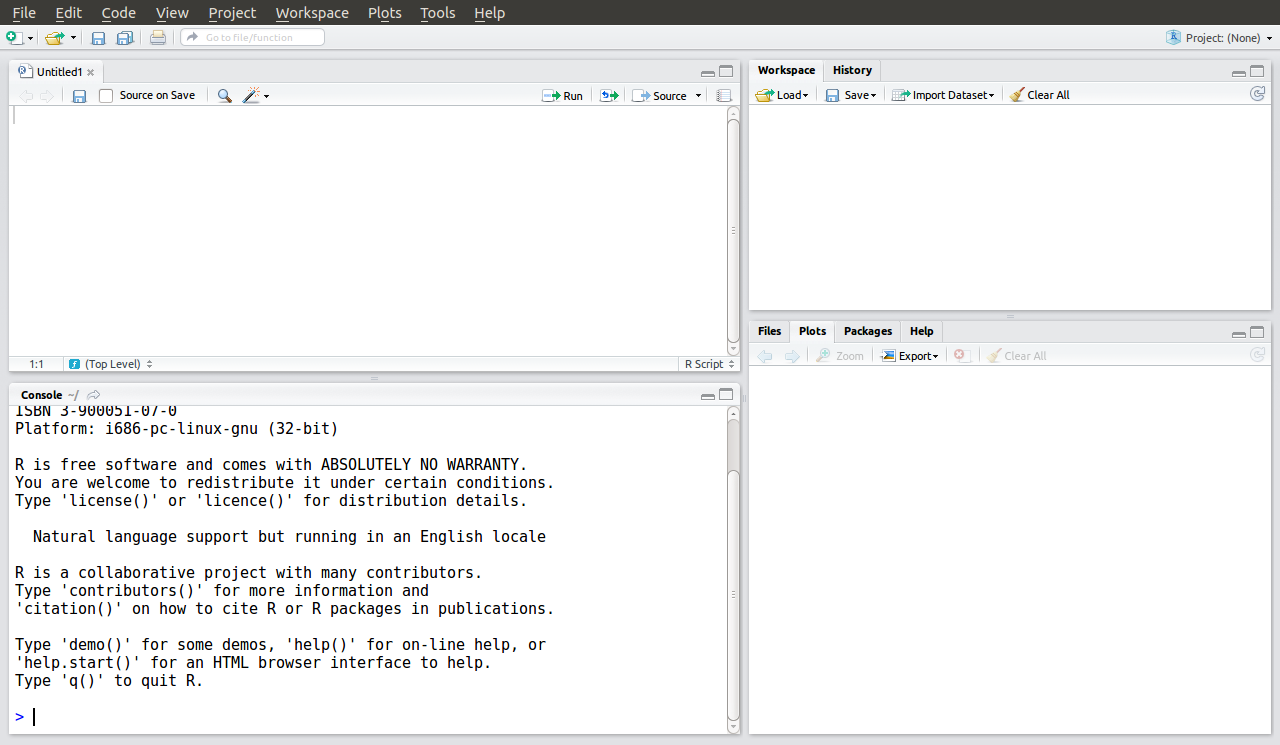
\includegraphics[width=\textwidth]{figure/RStudio_008}
\end{figure}

Essa parte superior é o editor de scripts, onde você pode digitar os
comandos do \R, e salvá-los para abrir depois em uma nova sessão. Para
salvar, clique no menu em \textsf{File $\rightarrow$ Save As...}, como
na figura abaixo:

\begin{figure}[H]
  \centering
  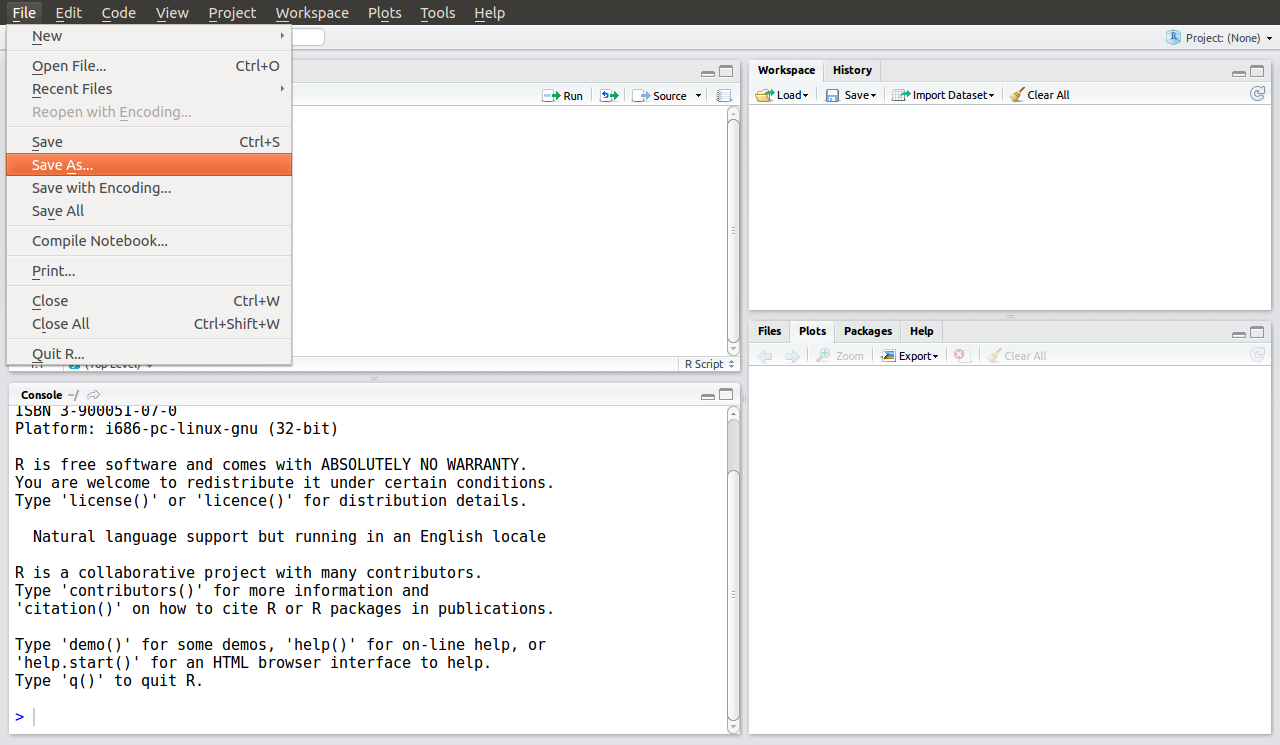
\includegraphics[width=\textwidth]{figure/RStudio_009}
\end{figure}

Na janela que abrir, digite o nome que você quer dar para o arquivo e
salve. Esse processo vai gerar um arquivo com extensão \texttt{.R} no
final (por exemplo \texttt{meu-script.R}), dentro do seu diretório de
trabalho (que você já definiu acima).

No editor de scripts, você digita os comandos que quiser, e quando
quiser executá-los no \textsf{Console}, seleciona uma linha (ou mais
linhas) e aperte as teclas \textsf{Ctrl+Enter}. O \RStudio se encarrega
de enviar esse comandos para serem executados.

Uma forma de organização dos seus scripts é adicionar comentários entre
comandos, o que facilita muito quando você for rever novamente esse
script, ou quiser enviar para outras pessoas. Você pode adicionar
comentários usando o símbolo \texttt{\#} na frente de qualquer frase que
não seja um comando. Por exemplo:

\begin{knitrout}\small
\definecolor{shadecolor}{rgb}{0.969, 0.969, 0.969}\color{fgcolor}\begin{kframe}
\begin{alltt}
\hlstd{> }\hlcom{# isso é um comentário e não será executado pelo R}
\hlstd{> }\hlstd{x} \hlkwb{<-} \hlnum{2} \hlopt{+} \hlnum{2}
\hlstd{> }\hlstd{y} \hlkwb{<-} \hlnum{4} \hlopt{*} \hlnum{4} \hlcom{# comentários também podem ser colocados ao lado de comandos}
\hlstd{> }\hlcom{# use esse recurso para descrever o que está sendo feito}
\hlstd{> }\hlcom{# o comando abaixo serve para listar os objetos criados}
\hlstd{> }\hlkwd{ls}\hlstd{()}
\end{alltt}
\end{kframe}
\end{knitrout}

Para ajuda com o \RStudio, você pode clicar na aba \texttt{Help} do
\RStudio (no quadro inferior direito) para ir se familiarizando com o
programa. Se você quiser ir se familiarizando com a linguagem em si,
digite
\begin{knitrout}\small
\definecolor{shadecolor}{rgb}{0.969, 0.969, 0.969}\color{fgcolor}\begin{kframe}
\begin{alltt}
\hlstd{> }\hlkwd{help.start}\hlstd{()}
\end{alltt}
\end{kframe}
\end{knitrout}
\noindent para ter acesso aos manuais e outras referências. Para uma boa
referência inicial em português recomendo seguir o material e os
exemplos de ``Introdução ao Ambiente Estatístico R'', do Prof. Paulo
Justiniano Ribeiro Jr. nesse link
\url{http://leg.ufpr.br/~paulojus/embrapa/Rembrapa/}

%% \section{Configurando o diretório de trabalho}

%% Antes de abrir o programa, a primeira coisa a fazer é configurar um
%% \emph{diretório de trabalho}, onde os arquivos que iremos utilizar serão
%% salvos. Para isso, clique com o botão direito do mouse sobre um ícone do
%% \R\ e depois em \textsf{Propriedades}. Clique na aba \textsf{Atalho},
%% procure pelo campo \textsf{Iniciar em:} e coloque todo o caminho da
%% pasta que deseja trabalhar. Por exemplo, se vamos usar a pasta
%% \verb|C:\Meus documentos|, sua configuração deve ficar como demonstrado
%% na Figura \ref{fig:propr}.

%% \section{Operações e comandos básicos}

%% \begin{itemize}
%% \item[a.] Faça uma operação simples e observe o resultado:
%% \begin{verbatim}
%% > 2+2
%% \end{verbatim}

%% \item[b.] Armazene o resultado de uma operação simples em um objeto
%%   \texttt{x} e observe este objeto:
%% \begin{verbatim}
%% > x <- 2+2
%% > x
%% \end{verbatim}

%% \item[c.] Crie um novo objeto \texttt{y} utilizando o objeto \texttt{x}:
%% \begin{verbatim}
%% > y <- x*3
%% > y
%% \end{verbatim}

%% \item[d.] Observe os objetos criados na área de trabalho:
%% \begin{verbatim}
%% > ls()
%% \end{verbatim}

%% \item[e.] Como os objetos \texttt{x} e \texttt{y} são apenas exemplos,
%%   vamos removê-los da área de trabalho:
%% \begin{verbatim}
%% > rm(x, y)
%% \end{verbatim}
%% \end{itemize}

%% \section{Entrada de dados}

%% \begin{itemize}
%% \item[a.] Entrada manual de um vetor com a função \texttt{c()}:
%% \begin{verbatim}
%% > dados1 <- c(5, 4, 2, 5, 6, 8, 6, 7, 5, 3)
%% > dados1
%% \end{verbatim}

%% \item[b.] Entrada manual de uma matriz com a função \texttt{matrix()}:
%% \begin{verbatim}
%% > dados2 <- matrix(c(6, 4, 5, 8, 7, 8, 2, 5, 4, 4, 5, 6), ncol=3, nrow=4)
%% > dados2
%% \end{verbatim}

%% \item[c.] Use a função \texttt{edit()} para criar um \textit{data frame}
%%   com os mesmos valores da matriz acima:
%% \begin{verbatim}
%% > dados3 <- edit(data.frame())
%% > dados3
%% \end{verbatim}

%% \item[d.] Use a função \texttt{read.table()} para importar a base de
%%   dados \texttt{carangueijos.xls} do Excel:
%%   \begin{itemize}
%%   \item[d.1.] Abra o arquivo no Excel e salve com o mesmo nome, mas
%%     utilizando a extensão \texttt{csv} (\textit{comma separated values}
%%     ou texto separado por vírgula).
%%   \item[d.2.] No \R\ importe o arquivo com:
%% \begin{verbatim}
%% > dados4 <- read.table("carangueijos.csv", header = TRUE, sep = ";",
%% + dec = ",")
%% \end{verbatim}
%% NOTA: os argumentos \texttt{sep} e \texttt{dec} podem mudar para
%% \verb|","| e \verb|"."| respectivamente, se o Excel estiver configurado
%% em inglês.
%%   \end{itemize}
%% \end{itemize}

%% \section{Comandos para resumo dos dados e estatística descritiva}

%% \begin{itemize}
%% \item[a.] Verifica as classes e a dimensão dos objetos criados:
%% \begin{verbatim}
%% # classe (repita para os outros objetos)
%% > class(dados1)
%% # dimensão (comprimento) de vetores (uma dimensão)
%% > length(dados1)
%% # para matrizes e data frames (duas ou mais dimensões)
%% > dim(dados2)
%% > dim(dados4)
%% \end{verbatim}

%% \item[b.] Verifica a estrutura dos objetos (repita para todos):
%% \begin{verbatim}
%% > str(dados1)
%% \end{verbatim}

%% \item[c.] Comandos básicos para o cálculo de estatísticas:
%% \begin{verbatim}
%% > min(dados1); max(dados1)
%% > mean(dados1); median(dados1)
%% > sd(dados1); var(dados1)
%% \end{verbatim}

%% \item[d.] Veja um resumo das informações com a função \texttt{summary}
%%   (repita para todos):
%% \begin{verbatim}
%% > summary(dados1)
%% \end{verbatim}
%% \end{itemize}

%% \section{Indexação e seleção condicional}

%% \begin{itemize}
%% \item[a.] Para indexar um vetor (i.e. selecionar uma posição) usam-se
%%   colchetes:
%% \begin{verbatim}
%% # segundo elemento de dados1
%% > dados1[2]
%% # os quatro primeiros elementos
%% > dados1[1:4]
%% \end{verbatim}

%% \item[b.] Para indexar matrizes e \textit{data frames} deve-se
%%   especificar a posição de linhas e colunas:
%% \begin{verbatim}
%% # elemento da segunda linha da terceira coluna de dados2
%% > dados2[2,3]
%% # as três primeiras linhas da primeira coluna
%% > dados2[1:3,1]
%% # todas as linhas da terceira coluna de dados3
%% > dados3[,3]
%% # data frames também podem ser indexados pelo nome das colunas
%% > dados4[1:10, "LF"]
%% # incluindo mais de uma coluna
%% > dados4[1:10, c("LF", "LC")]
%% \end{verbatim}

%% \item[c.] Para acessar apenas uma coluna de um \textit{data frame}
%%   usamos \verb|$|:
%% \begin{verbatim}
%% # todos os valores da coluna LC
%% > dados4$LC
%% \end{verbatim}

%% \item[d.] Através da indexação também podemos selecionar valores de
%%   acordo com algum critério:
%% \begin{verbatim}
%% # valores de LC maiores que 45
%% > dados4$LC[dados4$LC > 45]
%% # para mostrar todas as colunas que satisfazem a condição acima
%% > dados4[dados4$LC > 45,]
%% # colunas onde LC maior que 45 e somente para a espécie azul
%% > dados4[dados4$LC > 45 & dados4$spp == "Azul",]
%% # colunas onde LC maior que 45 ou onde a espécie seja azul
%% > dados4[dados4$LC > 45 | dados4$spp == "Azul",]
%% \end{verbatim}
%% \end{itemize}

%% \section{Gráficos}

%% \begin{itemize}
%% \item[a.] Gráfico para explorar uma base de dados:
%% \begin{verbatim}
%% > plot(dados4)
%% \end{verbatim}

%% \item[b.] Gráficos de dispersão:
%% \begin{verbatim}
%% # LC x CC
%% > plot(dados4$LC, dados4$CC)
%% # alterando nome dos eixos e tipo de ponto
%% > plot(dados4$LC, dados4$CC, xlab = "Largura da carapaça (mm)",
%% + ylab = "Comprimento da carapaça (mm)", pch = 3)
%% # alterando também os limites dos eixos e adicionando título
%% > plot(dados4$LC, dados4$CC, xlab = "Largura da carapaça (mm)",
%% + ylab = "Comprimento da carapaça (mm)", pch = 3, xlim = c(10, 60),
%% + ylim = c(10, 50), main = "Relação entre LC e CC")
%% \end{verbatim}

%% \item[c.] Diagramas de caixa:
%% \begin{verbatim}
%% # boxplot de LC
%% > boxplot(dados4$LC)
%% # todas as medidas lado a lado
%% > boxplot(dados4[,3:7], xlab = "Medidas", ylab = "Milimetros")
%% # boxplot de LC separado por espécie
%% > boxplot(LC ~ sexo, data = dados4, xlab = "Sexo",
%% + ylab = "Largura da carapaça (mm)")
%% # separado por espécie e sexo
%% > boxplot(LC ~ spp + sexo, data = dados4, xlab = "Espécie e Sexo",
%% + ylab = "Largura da carapaça (mm)")
%% \end{verbatim}

%% \item[d.] Histogramas:
%% \begin{verbatim}
%% # histograma de LC
%% > hist(dados4$LC)
%% # alterando a divisão de classes para 2 mm e outros parâmetros
%% # gráficos
%% > hist(dados4$LC, breaks = seq(16, 56, 2), xlim = c(10,60),
%% + xlab = "Largura da carapaça (mm)", ylab = "Frequência",
%% + main = "Histograma da largura da carapaça", col = "gray")
%% # salve uma saída de histograma em um objeto e observe o resultado
%% > h <- hist(dados4$LC, breaks = seq(16, 56, 2))
%% > h
%% \end{verbatim}
%% \end{itemize}

%% \section{Correlação e regressão (?)}

%% \section{Salvando gráficos}

%% Existem pelo menos três formas diferentes de salvar gráficos no \R:
%% \begin{enumerate}
%% \item Clicando com o botão direito do mouse sobre a figura existe a
%%   opção \textsf{Salvar como Metafile}, que salva a figura com a extensão
%%   \texttt{emf}.  Também existem as opções de apenas copiar, como Metafile
%%   ou Bitmap (\texttt{bmp}). É importante ressaltar que o tamanho da
%%   figura salva será idêntico ao que está aparecendo na tela.

%% \item Clicando sobre a figura, vá no menu \textsf{Arquivo > Salvar
%%   como...} e uma série de opções de formatos de figuras deverão
%%   aparecer. Escolha o formato desejado e salve. Assim como no caso
%%   acima, o tamanhho da figura será o mesmo que está na tela.

%% \item Uma forma mais eficiente de salvar as figuras é através das
%%   funções próprias do \R\ para essa finalidade. As principais funções
%%   são \texttt{bmp()}, \texttt{png()}, \texttt{jpeg()} e
%%   \texttt{pdf()}, para gerar arquivos de figura com as extensões
%%   \texttt{bmp}, \texttt{png}, \texttt{jpeg} e \texttt{pdf}
%%   respectivamente. Por exemplo, para salvar uma das figuras feitas acima
%%   em \texttt{bmp}, por exemplo, podemos fazer:
%% \begin{verbatim}
%% > bmp("Figura_LC_CC.bmp")
%% > plot(dados4$LC, dados4$CC, xlab = "Largura da carapaça (mm)",
%% + ylab = "Comprimento da carapaça (mm)", pch = 3)
%% > dev.off()
%% \end{verbatim}
%% Note que sempre que utilizar alguma dessas funções para gerar figuras,
%% \emph{obrigatoriamente} você deverá utilizar a função \texttt{dev.off()}
%% quando terminar o código da figura. Caso contrário ela não será salva no
%% arquivo.

%% A maior vantagem deste método é que o tamanho das figuras pode ser
%% especificado explicitamente, e portanto, todas as figuras são geradas
%% com exatamente o mesmo tamanho. Por exemplo, para gerar a mesma figura
%% com 15 cm da largura (\texttt{width}) por 15 cm de altura
%% (\texttt{height}) podemos fazer:
%% \begin{verbatim}
%% > bmp("Figura_LC_CC.bmp", width = 15, height = 15, units = "cm", res = 72)
%% > plot(dados4$LC, dados4$CC, xlab = "Largura da carapaça (mm)",
%% + ylab = "Comprimento da carapaça (mm)", pch = 3)
%% > dev.off()
%% \end{verbatim}

%% \end{enumerate}

%% \section{Finalizando o programa e salvando a área de trabalho}

%% \begin{itemize}
%% \item[a.] No \textsf{R} clique em \textsf{Arquivo} e depois em
%%   \textsf{Salvar área de trabalho...}.
%% \item[b.] Na janela que abrir verifique se a pasta que está aparecendo é
%%   a mesma que você direcionou no início da aula.
%% \item[c.] No campo \textsf{Nome do arquivo:} irá aparecer o nome
%%   \texttt{.RData}. Não é necessário modificar este nome. Clique no botão
%%   \textsf{Salvar}.
%% \end{itemize}


\end{document}
